\documentclass[a4paper, 11pt]{article}
\usepackage{geometry}
\geometry{letterpaper, margin=1in}
\usepackage{graphicx}
\graphicspath{ {images/} }

\usepackage{amsmath}
\usepackage{amssymb}  
\usepackage{amsthm}
\usepackage{ulem}

\usepackage{enumitem}


\usepackage{pdfpages} % for including full pdf pages

\usepackage{empheq}

\usepackage{listings}


%format to allow bolded theorems, corollaries, etc...
\newtheorem*{theorem}{Theorem}
\newtheorem*{corollary}{Corollary}
\newtheorem*{lemma}{Lemma}
\newtheorem*{definition}{Definition}
\newtheorem*{Example}{Example} 
\newtheorem*{Remark}{Remark}

% stop typing \mathbb a thousand times 
\newcommand{\R}{\mathbb{R}}
\newcommand{\C}{\mathbb{C}}
\newcommand{\F}{\mathbb{F}}
\newcommand{\E}{\mathcal{E}}
\newcommand{\prob}[2]{\mathcal{P}_{_{#1\rightarrow #2}}}
\newcommand{\M}{\mathbb{M}}
\newcommand{\sphere}{\mathbb{S}}

% commands for bra-ket notation
\newcommand{\bra}[1]{\ensuremath{\left\langle#1\right|}}
\newcommand{\ket}[1]{\ensuremath{\left|#1\right\rangle}}
\newcommand{\bracket}[2]{\ensuremath{\left\langle #1 \middle| #2 \right\rangle}}
\newcommand{\matrixel}[3]{\ensuremath{\left\langle #1 \middle| #2 \middle| #3 \right\rangle}}
\newcommand{\expectation}[1]{\ensuremath{\left\langle #1 \right\rangle}}

% vector stuff
\newcommand{\basis}[1]{\hat{\mathbf{e}}_#1}
\newcommand{\unit}[1]{\hat{\boldsymbol{#1}}}
\newcommand{\bvec}[1]{\vec{\boldsymbol{#1}}}
\newcommand{\threevec}[2]{\begin{pmatrix} #1 \\ #2 \end{pmatrix}}

% change margins for solution
\newenvironment{solution}{%
	\begin{list}{}{%
			\setlength{\topsep}{0pt}%
			\setlength{\leftmargin}{0.5cm}%
			\setlength{\rightmargin}{0.5cm}%
			\setlength{\listparindent}{\parindent}%
			\setlength{\itemindent}{\parindent}%
			\setlength{\parsep}{\parskip}%
		}%
		\item[]}{\end{list}}




\begin{document}
\noindent
\large\textbf{Homework 2} \hfill \textbf{John Waczak} \\
\normalsize PH 653 \hfill  Date: \today \\
Dr. Oksana Ostroverkhova \hfill worked w/ Ryan Tollefsen
\par\noindent\rule{\textwidth}{0.4pt} \\\\



\begin{enumerate}[leftmargin=0em, label=\textbf{\arabic*}]
  \item Consider a 1D harmonic oscillator of mass $m$, angular frequency
    $\omega_0$ and charge $q$. Let $\ket{n}$ be eigenstates of the Hamiltonian
    $H_0$. For $t<0$, the oscillator is in the ground state $\ket{0}$. At $t=0$,
    it is subjected to an electric field pulse of amplitude $\E$ and duration
    $\tau$. Let $\prob{0}{n}$ be the probability of finding the oscillator in
    the state $\ket{n}$ after the pulse.

    \begin{enumerate}[leftmargin=2em, label=(\textbf{\alph*})]
    \item Write down the time-dependent perturbation to $H_0$.\\
      \begin{solution}
        Recall that the electric field is related to the electric potential by
        \begin{equation}
          \bvec{E} = -\nabla \Phi
        \end{equation}
        From the above problem statement, we must have that after turning on,
        the electric field is of the form
        \begin{equation}
          \bvec{E} = \E\unit{x} 
        \end{equation}
        where I have chosen $x$ as the distance parameter. The potential energy
        $V$ due to a charge $q$ in an electric potential $\Phi$ is just $q\Phi$
        and therefore, the complete perturbation potential may be written as
        \begin{equation}
          V(x,t) = \begin{cases}
            -qx\E & 0\leq t\leq \tau \\
            0 & \text{otherwise}
          \end{cases}
        \end{equation}
      \end{solution}
      
    \item Calculate $\prob{0}{1}$ by using first order time-dependent
      perturbation theory. How does $\prob{0}{1}$ vary with $\tau$ for fixed
      $\omega_0$?\\
      \begin{solution}
        The first order, coupled differential equations for the coefficients
        through the second order are
        \begin{align}
          \lambda^0:\qquad &\i\hbar\frac{d}{dt}c_n^0(t) = 0 \\
          \lambda^1:\qquad &i\hbar\frac{d}{dt}c_n^1(t) = \sum_k V_{nk}(t)c_k^0(t)e^{i\omega_{nk}t}\\
          \lambda^2:\qquad &i\hbar\frac{d}{dt}c_n^2(t) = \sum_k V_{nk}(t)c_k^1(t)e^{i\omega_{nk}t}
        \end{align}
        Each of these differential equations is separable in $t$ and recursively
        requires the previous order correction. So long as $\ket{i}\neq\ket{f}$
        (as is the case for parts b and c of this problem), then the first order
        correction is given by
        \begin{equation}
          c_f^1(t)= \frac{1}{i\hbar}\int_{t_0}^t V_{fi}(t')e^{i\omega_{fi}t'}dt'
        \end{equation}
        which leads to a first order probability approximation given by
        \begin{equation}
          \prob{i}{f}\approx \frac{1}{\hbar^2}\left| \int_{t_0}^t V_{fi}(t')e^{i\omega_{fi}t'}dt'\right|^2 
        \end{equation}
        To calculate this integral, we must first evaluate the matrix element in
        question. We have that $i=0$ and $f=1$ so that the matrix element is
        given by
        \begin{align}
          V_{10}(t) &= \matrixel{1}{V(t)}{0} \\
                    &= \matrixel{1}{-qx\E}{0} \\
                    &= -q\E\matrixel{1}{x}{0} 
        \end{align}
        Recall from PH651 that the ladder operator representation of the
        position operator is
        \begin{equation}
          x = \sqrt{\frac{\hbar}{2m\omega_0}}\Big(a+a^\dagger \Big)
        \end{equation}
        where
        \begin{align}
          a\ket{n} &= \sqrt{n}\ket{n-1} \\
          a^\dagger\ket{n} &= \sqrt{n+1}\ket{n+1}
        \end{align}
        returning to the problem, we now have that
        \begin{align}
          V_{10}(t) &= -q\E\sqrt{\frac{\hbar}{2m\omega_0}}\matrixel{1}{\left(a+a^\dagger\right)}{0} \\
                    &=-q\E\sqrt{\frac{\hbar}{2m\omega_0}}\bracket{1}{1}\\
          &= -q\E\sqrt{\frac{\hbar}{2m\omega_0}}
        \end{align}
        In fact, the matrix element does not depend on $t$. It follows that the
        probability is given by
        \begin{align}
          \prob{0}{1} &= \frac{1}{\hbar^2}\left|\int_{t_0}^t-q\E\sqrt{\frac{\hbar}{2m\omega_0}}e^{i\omega_{10}t'}dt'  \right|^2\\
                      &=\frac{q^2\E^2}{2m\hbar\omega_0}\left|\int_{t_0}^te^{i\omega_{10}t'}dt'  \right|^2\\
          \omega_{10} &= \left( \hbar\omega_0\frac{3}{2}-\hbar\omega_0\frac{1}{2} \right) = \omega_0 \\
          \Rightarrow \prob{1}{0} &= \frac{q^2\E^2}{2m\hbar\omega_0}\left|\int_{0}^\tau e^{i\omega_{0}t'}dt'  \right|^2\\
                      &= \frac{q^2\E^2}{2m\hbar\omega_0}\left|\frac{1}{i\omega_ 0}(e^{i\omega_0\tau}-1)\right|^2\\
                      &= \frac{q^2\E^2}{2m\hbar\omega_0}\left|\frac{e^{i\omega_0\tau/2}}{i\omega_0}(e^{i\omega_0\tau/2}-e^{-i\omega_0\tau/2})\right|^2\\
                      &= \frac{q^2\E^2}{2m\hbar\omega_0}\left|\frac{e^{i\omega_0t/2}}{i\omega_0}2\sin(\omega_0\tau/2)\right|^2\\
                      &= \frac{2q^2\E^2}{m\hbar\omega_0^3}\sin^2(\omega_0\tau/2)\\
        \end{align}
        From this we can see that the probability is oscillatory in $\tau$. This 
      \end{solution}
      
    \item Show that, to obtain $\prob{0}{2}$, the calculation must be done at
      least to the second order. Calculate $\prob{0}{2}$ to this order. \\
      \begin{solution}
        In order to calculate the first order approximation, we need to
        determine the matrix element $V_{20}$. However, because $x$ can be
        written in terms of raising and lowering operators, this matrix element
        must be zero as is shown below:
        \begin{align}
          V_{20} &= -q\E\sqrt{\frac{\hbar}{2m\omega_0}}\matrixel{2}{\left(a+a^\dagger\right)}{0} \\
                 &=  -q\E\sqrt{\frac{\hbar}{2m\omega_0}}\bracket{2}{1} \\
                 &= 0
        \end{align}
        Therefore, we require the second order perturbation to determine the
        probability. Combining equation 7 with equation 6 yields
        \begin{equation}
          i\hbar \frac{d}{dt}c_n^2(t) = \sum_k V_{nk}e^{i\omega_{nk}t}\frac{1}{i\hbar}\int_0^\tau V_{k i}e^{i\omega_{ki}t}dt
        \end{equation}
        Again, this equation is separable in $t$ and can therefore be integrated
        to obtain the second order coefficients
        \begin{align}
          c_{f}^2(t) &= -\frac{1}{\hbar^2}\sum_k\int_0^\tau dt'\;  V_{fk}(t')e^{i\omega_{fk}t'}\int_0^t dt'' \; V_{ki}(t'')e^{i\omega_{ki}t''} 
        \end{align}
        For this problem, $f=2$ and $i=0$. We therefore care about the matrix
        elements $V_{2k}$ and $V_{k0}$. From both of our previous arguments, it
        is clear that the only surviving term in the series is for $k=2$ as it
        is the only term for which $V_{fk}$ and $V_{ki}$ are not both zero.
        Thus, we have
        \begin{align}
          c_2^2(t) &= -\frac{1}{\hbar^2}\left(-q\E \sqrt{\frac{\hbar}{2m\omega_0}} \right)^2\int_0^\tau dt'\;\matrixel{2}{a+a^\dagger}{1}  e^{i\omega_0 t'}\int_0^{t'}dt''\; e^{i\omega_0 t''} \\
                   &= -\frac{q^2\E^2}{2m\omega_0\hbar}\sqrt{2} \int_0^\tau dt'\; e^{i\omega_0 t'}\int_0^{t'}dt''\; e^{i\omega_0 t''} \\
                   &= -\frac{q^2\E^2}{\sqrt{2}m\omega_0\hbar} \int_0^\tau dt'\; e^{i\omega_0 t'}\left( \frac{1}{i\omega_0}(e^{i\omega_0 t'}-1) \right) \\
                   &= -\frac{q^2\E^2}{\sqrt{2}m\omega_0\hbar} \int_0^\tau dt'\; \left( \frac{1}{i\omega_0}(e^{2i\omega_0 t'}-e^{i\omega_0 t'}) \right) \\
                   &= -\frac{q^2\E^2}{\sqrt{2}m\omega_0\hbar}\left( -\frac{\left( e^{i\omega_o\tau}-1 \right)^2}{2\omega_0} \right) \\
                   &= \frac{q^2\E^2}{m\omega_0^32\hbar\sqrt{2}}\left( e^{i\omega_o\tau}-1 \right)^2 \\
                   &= \frac{2q^2\E^2e^{i\omega_0\tau}}{m\omega_0^3\hbar\sqrt{2}}\sin^2(\omega\tau/2) 
        \end{align}
        and therefore, the probability is given by
        \begin{align}
          \prob{0}{2} &= |c_2^1(t)_2^2(t)|^2 \\
                      &= |0+c_2^2(t)|^2 \\
          &= \frac{2q^4\E^4}{m^2\omega^6\hbar^2}\sin^4(\omega\tau/2)
        \end{align}
      \end{solution}
    \end{enumerate}
    
  \item A hydrogen atom is in the ground state at $t=-\infty$. An electric field
    $\bvec{E}(t)=\unit{k}\E e^{-t^2/\tau^2}$ is applied until $t=+\infty$. What
    is the probability that the atom ends up in any of the $n=2$ states to the
    first order? Does this answer depend on whether or not we incorporate spin
    in the picture? \\
    \begin{solution}
      Given the time-varying electric field from above, the corresponding
      perturbation potential is given by
      \begin{equation}
        V(z,t)= -zq\E e^{-t^2/\tau^2}
      \end{equation}
      where I have made the assumption that $\unit{k}=\unit{z}$. Because the
      hydrogen atom is spherically symmetric, this choice should not affect our
      answer. There are four possible $n=2$ states, namely one $2s$ state and
      three $2p$ states. We therefore must calculate the following matrix
      elements
      \begin{equation}
        \matrixel{200}{V(t)}{100}\qquad\matrixel{210}{V(t)}{100}\qquad\matrixel{21\pm 1}{V(t)}{100}
      \end{equation}
      As an operator, we may identify
      \begin{equation}
        z = \sqrt{\frac{4\pi}{3}}rY_1^0 = \sqrt{\frac{4\pi}{3}}rT_0^{(1)}
      \end{equation}
      or, in other words, $z$ can be thought of as a first rank spherical tensor
      operator. Then, the Wigner-Eckart theorem gives the selection rule that
      $m'=q+m$. Here $q=0$ and $m=0$ so that we can immediately say
      \begin{equation}
        \matrixel{211}{V}{100}=0 \qquad \matrixel{21-1}{V}{100}=0
      \end{equation}

      We can also see that $\matrixel{200}{V}{100}=0$ as the angular portion of
      the integral will look like
      \begin{equation}
        \int d\Omega \left(Y_0^0\right)^*Y_1^0Y_0^0
      \end{equation}
      and must be zero due to parity.  That leaves just 1 final element which we
      can directly integrate
      \begin{align}
        \matrixel{210}{V}{100} &= -q\E e^{-t^2/\tau^2}\matrixel{210}{z}{100} \\
                               &= -q\E e^{-t^2/\tau^2}\matrixel{210}{\sqrt{\frac{4\pi}{3}}rY_1^0}{100}\\
                               &= -q\E e^{-t^2/\tau^2}\left(\frac{128\sqrt{2}a_0}{243}\right)
      \end{align}
      where the last calculation was performed using Mathematica. The
      probability is therefore given by
      \begin{align}
        \prob{gs}{n=2} &= \frac{1}{\hbar^2}\left(\frac{128\sqrt{2}a_0}{243}\right)^2\left| \int_{-\infty}^{\infty}-q\E e^{-t^2/\tau^2} e^{i\omega_{210,100}t} dt \right|^2\\
                       &= \frac{q^2\E^2}{\hbar^2}\left(\frac{128\sqrt{2}a_0}{243}\right)^2\left| \int_{-\infty}^{\infty} e^{-t^2/\tau^2} e^{i\omega_{210,100}t} dt \right|^2 \\
        &= \frac{2^{15}}{3^{10}}\frac{a_0^2 q^2 \E^2}{\hbar^2}\tau^2\pi e^{-\omega^2\tau^2/2}
      \end{align}
      The calculations for which are shown on the following Mathematica
      worksheet.

      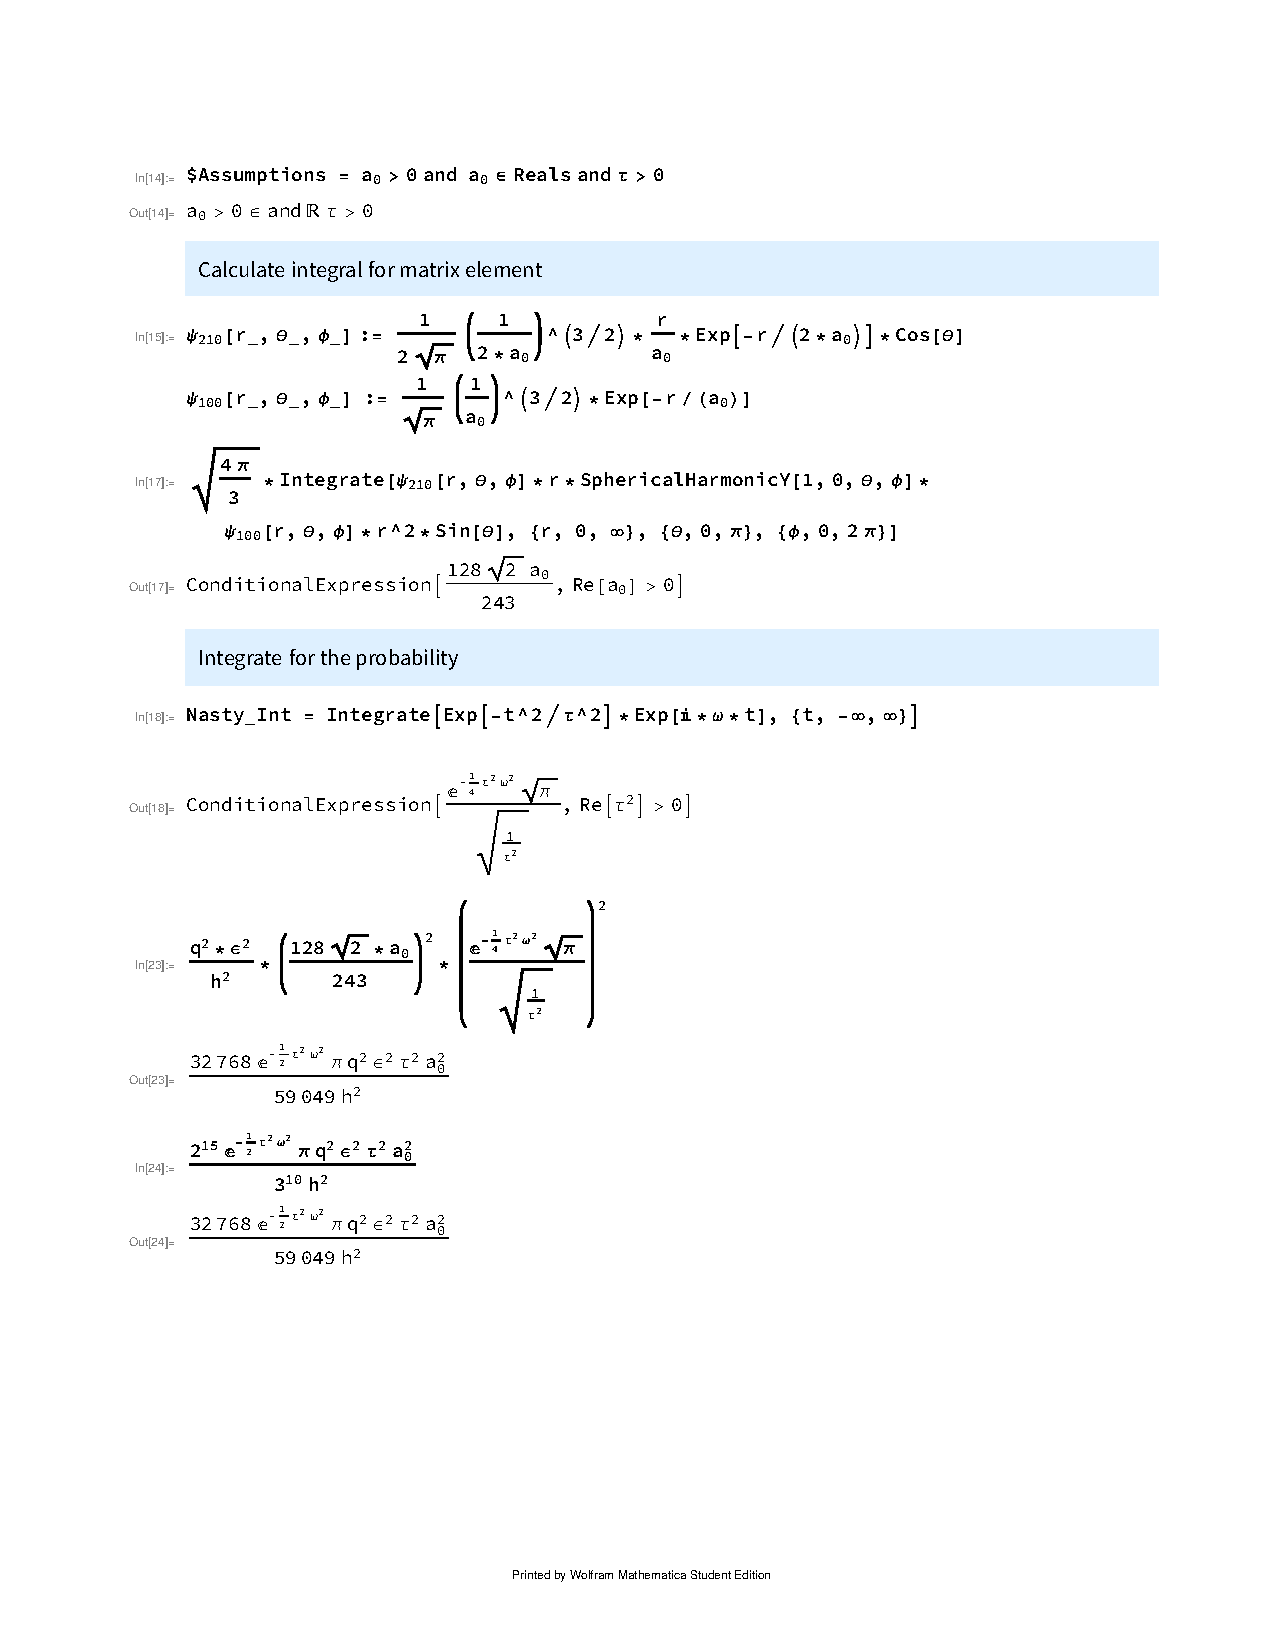
\includepdf{problem_2.pdf}

      Does this change if we consider the spin interaction? If we add spin to
      the picture, our states will now include a spin component:
      \begin{equation}
        \ket{n,\ell,m_\ell}\rightarrow \ket{n, \ell, m_\ell,s,m_s}
      \end{equation}
      But even with these new quantum numbers to consider, the spherical
      harmonic tensor operator $Y_1^0$ associated with the $z$ operator still
      only acts on the position space $\E_{\vec{r}}$ and consequently, none of our
      previous work will change. However, we know that if we consider the spin
      of the electron as forming a small current loop, then we can define a
      magnetic moment $\bvec{\mu}$. Although this $\bvec{\mu}$ does not interact
      directly with $\bvec{E}$, it does interact with the magnetic field. 
      \begin{equation}
        V = -\bvec{\mu}\cdot \bvec{B}
      \end{equation}
      we can expand the above equation further by identifying the relationship
      between electron spin and the magnetic moment, that is
      \begin{equation}
        V = g\frac{e}{2m}\bvec{S}\cdot \bvec{B}
      \end{equation}
      In order to tell if this interaction takes place, we must try and figure out
      what $\bvec{B}$ is. Recall that Faraday's law in differential form gives
      \begin{equation}
        \nabla\times\bvec{E} = -\frac{\partial}{\partial t}\bvec{B}  
      \end{equation}
      However, we have that
      \begin{equation}
        \bvec{E}(t) = \unit{k}\E e^{-t^2/\tau^2}
      \end{equation}
      which is a constant vector field in space for a given time $t$. Based on
      this fact,
      \begin{equation}
        \nabla\times\bvec{E} = (\nabla\times\unit{k})\E e^{-t^2/\tau^2} = 0
      \end{equation}
      and, therefore, $\bvec{B}$ must be constant in time. This result suggests
      that the interaction would be time independent and looks just like the
      Zeeman effect. 
    \end{solution}
    
   \item A 1D harmonic oscillator is in the state $n=0$ at $t=-\infty$. The
     perturbation is applied from $t=-\infty$ to $t=+\infty$. Show that if
     \begin{equation}
       V(t) = -e\E x/\left[ 1+(t/\tau)^2 \right],
     \end{equation}
    then to the first order,
    $\prob{0}{1}=\frac{e^2\E^2\pi^2\tau^2}{2m\omega\hbar}e^{-2\omega\tau}$

    \begin{solution}
      In order to find the first order correction, we first need to find the
      matrix element $V_{10}$ which is given by
      \begin{align}
        V_{10}(t) &= -\frac{e\E}{1+(t/\tau)^2}\matrixel{1}{x}{0}\\
                  &= -\frac{e\E}{1+(t/\tau)^2}\sqrt{\frac{\hbar}{2m\omega}}\matrixel{1}{a+a^\dagger}{0}\\
                  &= -\frac{e\E}{1+(t/\tau)^2}\sqrt{\frac{\hbar}{2m\omega}}
      \end{align}
      Using this, the probability of transitioning is given by
      \begin{align}
        \prob{0}{1} &= \frac{1}{\hbar^2}\left|\int_{-\infty}^\infty  V_{10}(t)e^{i\omega t}dt   \right|^2 \\
                    &= \frac{e^2\E^2}{2\hbar m\omega}\left|\int_{-\infty}^\infty  \frac{e^{i\omega t}}{1+(t/\tau)^2}dt   \right|^2 \\
      \end{align}
      This integral is not solvable by ordinary methods, however, as math gurus
      we can recognize that the denominator may be factored over the complex
      numbers yielding
      \begin{equation}
        \int_{-\infty}^\infty \frac{e^{i\omega t}}{(1+i\frac{t}{\tau})(1-i\frac{t}{\tau})}dt
      \end{equation}
      so that over the complex numbers, this integral has two simple poles at
      $t=\pm i\tau$. To find the value of the integral, we may consider
      alternatively a contour in the complex plane as shown in the following
      image \\
      \begin{figure}[!hbt]
        \centering
        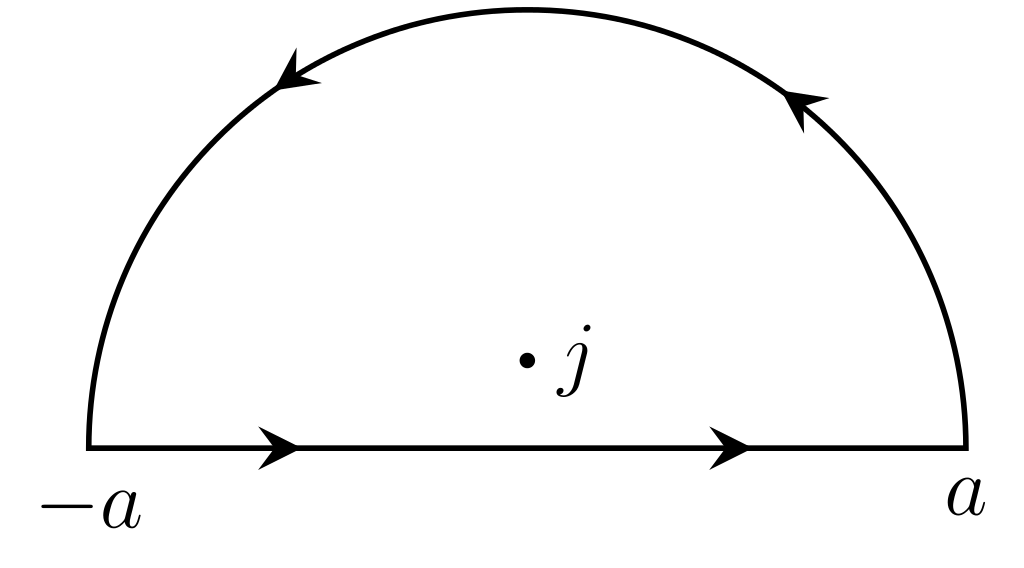
\includegraphics[width=0.5\columnwidth]{contour_integral}
        \caption{Contour integral in the complex plane showing one of the simple
        poles at the point $j=i\tau$}
      \end{figure}

      If we denote the path in the above figure as $C$ then,
      \begin{align}
        \oint_C \frac{e^{i\omega z}}{(1+i\frac{z}{\tau})(1-i\frac{z}{\tau})}dz &= 2\pi i\text{Res}(z=i\tau)\\
                                                                               &= 2\pi i \frac{-i\tau e^{-\omega\tau}}{2} \\
        &= \pi\tau e^{-\omega \tau}
      \end{align}
      We can also break up the path into two parts: the path along the real
      line, and the half circle. Our solution does not depend on $a$ and in the
      limit that $a\rightarrow \infty$ the integral along the half circle path
      vanishes so that
      \begin{equation}
        \int_{-\infty}^\infty \frac{e^{i\omega t}}{1+(t/\tau)^2}dt = \pi\tau e^{-\omega \tau}
      \end{equation}
      Plugging this into the equation for our probability yields

      \begin{align}
        \prob{0}{1} &=\frac{e^2\E^2}{2\hbar m\omega}\left| \pi\tau e^{-\omega \tau} \right|^2 \\
        &= \frac{e^2\E^2\pi^2\tau^2}{2\hbar m\omega}e^{-2\omega\tau}
      \end{align}
      which confirms the result! \\
    \end{solution}

    \item Consider a system containing two spin-$1/2$ particles. At $t=0$, the
      system is in the state $\ket{m_{s1}, m_{s2}}=\ket{+,-}$. The unperturbed
      Hamiltonian $H_0$ is spin-independent and can be taken as zero. At $t=0$,
      a time-independent perturbation is applied
      $V=\frac{4\Delta}{\hbar^2}\mathbf{S}_1\cdot\mathbf{S}_2$, where $S_1$ and
      $S_2$ are spin operators, and $\Delta$ is a constant.
      \begin{enumerate}[leftmargin=2em, label=(\textbf{\alph*})]
        \item Find the state of the system at an arbitrary time $t>0$.\\
          \begin{solution}
            We can re-write this perturbation to take advantage of the coupled
            basis.
            \begin{equation}
              V = \frac{2\Delta}{\hbar^2}\left( \bvec{S}^2-\bvec{S}_1^2-\bvec{S}_2^2 \right)
            \end{equation}
            At time $t=0$ we are in the state, $\ket{+,-}$ which in the coupled
            basis corresponds to
            \begin{equation}
              \ket{+,-} = \frac{1}{\sqrt{2}}(\ket{1,0}+\ket{0,0})
            \end{equation}
            Each component has its energy eigenvalue equation
            \begin{equation}
              V\ket{1,0} = \Delta \ket{1,0} \qquad V\ket{0,0}=-3\Delta\ket{0,0}
            \end{equation}
            which we can use to immediately write the time dependence, e.g.
            \begin{equation}
              \ket{\psi(t)} = \frac{1}{\sqrt{2}}\left(e^{-i\Delta t/\hbar}\ket{1,0}+e^{3i\Delta t/\hbar}\ket{0,0}  \right)
            \end{equation}
            
          \end{solution}

        
        \item Using the result of part (a), find the probabilities that after a
          time $t$ the system will end up in $\ket{+,+}$, $\ket{-,-}$,
          $\ket{+,-}$, and $\ket{-,+}$ states.
          \begin{solution}
            The probabilities are given by the squared norm of the coefficients
            of $\ket{\psi(t)}$ in the uncoupled basis, e.g.
            \begin{align}
              \mathcal{P}_{++} &= \left|\bracket{+,+}{\psi(t)}  \right|^2\\
                               &= \left| \bracket{1,1}{\psi(t)} \right|^2 = 0 \\
              \mathcal{P}_{--} &= \left| \bracket{-,-}{\psi(t)} \right|^2 \\
                               &=\left| \bracket{1,-1}{\psi(t)} \right|^2 = 0\\
              \mathcal{P}_{+,-} &= \left| (\bra{1,0}+\bra{0,0})\ket{\psi(t)} \right|^2 \\
                               &= \frac{1}{4}\left|  e^{-i\Delta t/\hbar}+e^{3i\Delta t/\hbar} \right|^2 \\
                               &= \frac{1+\cos(4\Delta t/\hbar)}{2} \\
              \mathcal{P}_{+,-} &= \left| (\bra{1,0}-\bra{0,0})\ket{\psi(t)} \right|^2 \\
                               &= \frac{1}{4}\left|  e^{-i\Delta t/\hbar}-e^{3i\Delta t/\hbar} \right|^2 \\
              &= \frac{1-\cos(4\Delta t/\hbar)}{2}
            \end{align}
            
            
          \end{solution}
          
          
        \item Now treat V as a perturbation (applied at $t=0$) and calculate
          the probabilities of the transitions described in part (b) using
          first-order perturbation theory.\\
          \begin{solution}
            To first order, the probability is given by
            \begin{equation}
              \prob{i}{f} = \left|c_f^0(t)+c_f^1(t)  \right|^2 = \left|\delta_{f,i}-\frac{i}{\hbar}\int_0^tV_{fi}(t')e^{i\omega_{fi}t'}dt'  \right|^2
            \end{equation}
            $V$ is clearly diagonal for the coupled states. Therefore, if our
            final state is either $\ket{+,+}=\ket{1,1}$ or
            $\ket{-,-}=\ket{1,-1}$ the probability must be zero by
            orthogonality. For the other two possibilities, we therefore have
            \begin{equation}
              \prob{i}{f} = \left|1- \frac{i}{\hbar} \int_0^t V_{f,i}(t')e^{i\omega_{fi}t'}dt' \right|^2 
            \end{equation}
            so that the probabilities become
            \begin{align}
              \mathcal{P}_{+,-} &= \left|1-\frac{i}{\hbar}\int_0^t \frac{1}{2}(\Delta\bracket{1,0}{1,0}-3\Delta\bracket{0,0}{0,0})e^{i0t'}dt'  \right|^2\\
                                &= \left| 1+\frac{i\Delta t}{\hbar} \right|^2 = 1+\frac{\Delta^2 t^2}{\hbar^2}\\
              \mathcal{P}_{-,+} &= \left|0-\frac{i}{\hbar}\int_0^t \frac{1}{2}(\Delta\bracket{1,0}{1,0}+3\Delta\bracket{0,0}{0,0})e^{i0t'}dt'  \right|^2\\
              &= \left|-\frac{i2\Delta t}{\hbar}  \right|^2 = \frac{4\Delta^2 t^2}{\hbar^2}
            \end{align}
            
              
          \end{solution}
          
        \item Compare the exact solution found in part (b) with the approximate
          one found in part (c) and comment.
          \begin{solution}
            The perturbation theory agrees exactly with the analytic solution
            for the two final states $\ket{+,+}$ and $\ket{-,-}$. This makes
            sense because if a state can never be reach it is unlikely that we
            can add successively smaller terms using a perturbation approach and
            reach a zero value. For the other two approximations, let's
            consider the Power series for our exact solutions

            \begin{align}
              \frac{1+\cos(4\Delta t/\hbar)}{2} &= \frac{1}{2}+\frac{1}{2}-\frac{1}{2}\left( \frac{16\Delta^2t^2}{2!\hbar^2} \right)\\
                                                &= 1-\frac{4\Delta^2t^2}{\hbar^2}\\
              \frac{1-\cos(4\Delta t/\hbar)}{2} &= \frac{1}{2}-\frac{1}{2}+\frac{1}{2}\left( \frac{16\Delta^2t^2}{2!\hbar^2} \right)\\
                                                &= \frac{4\Delta^2t^2}{\hbar^2}
            \end{align}
            
            Therefore, $\mathcal{P}_{+,-}$ is almost exact up to the coefficent
            of the $t^2$ term and $\mathcal{P}_{-,+}$ is exact. 

          \end{solution}
          
      \end{enumerate}
      
\end{enumerate}

  
\end{document}






























